\documentclass[journal,12pt,onecolumn]{IEEEtran}
\usepackage{cite}
\usepackage{amsmath,amssymb,amsfonts,amsthm}
\usepackage{algorithmic}
\usepackage{graphicx}
\usepackage{textcomp}
\usepackage{xcolor}
\usepackage{txfonts}
\usepackage{listings}
\usepackage{circuitikz}
\usepackage{enumitem}
\usepackage{mathtools}
\usepackage{gensymb}
\usepackage{comment}
\usepackage[breaklinks=true]{hyperref}
\usepackage{tkz-euclide} 
\usepackage{listings}
\usepackage{gvv}                                        
\usepackage[latin1]{inputenc}                                
\usepackage{color}                                            
\usepackage{array}                                            
\usepackage{longtable}                                       
\usepackage{calc}                                             
\usepackage{multirow}                                         
\usepackage{hhline}                                           
\usepackage{ifthen}                                           
\usepackage{lscape}
\usepackage{tabularx}
\usepackage{array}
\usepackage{float}
\usepackage{multicol}

\newtheorem{theorem}{Theorem}[section]
\newtheorem{problem}{Problem}
\newtheorem{proposition}{Proposition}[section]
\newtheorem{lemma}{Lemma}[section]
\newtheorem{corollary}[theorem]{Corollary}
\newtheorem{example}{Example}[section]
\newtheorem{definition}[problem]{Definition}
\newcommand{\BEQA}{\begin{eqnarray}}
\newcommand{\EEQA}{\end{eqnarray}}
\newcommand{\define}{\stackrel{\triangle}{=}}
\theoremstyle{remark}
\newtheorem{rem}{Remark}

% Marks the beginning of the document
\begin{document}
\bibliographystyle{IEEEtran}
\vspace{3cm}

\title{Assignment 5}
\author{DESABOINA SRI SATHWIK-AI24BTECH11007}
\maketitle
% Removed \newpage to avoid a blank first page
\bigskip

\renewcommand{\thefigure}{\theenumi}
\renewcommand{\thetable}{\theenumi}
\section*{GATE-2007:ME}
\subsection*{Section-A- Carry one mark each}
\begin{enumerate}
\item The minimum value of function $y = x^2$ in the interval $[1,5]$ is

	\hfill{(GATE-ME:2007)}
\begin{multicols}{4}
\begin{enumerate}
    \item 1
    \item 1
    \item 25
    \item undefined
\end{enumerate}
\end{multicols}

\item If a square matrix $A$ is real and symmetric, then the eigenvalues

	\hfill{(GATE-ME:2007)}

\begin{multicols}{2}
\begin{enumerate}
    \item are always real
    \item are always real and positive
    \item are always real and non-negative
    \item occur in complex conjugate pairs
\end{enumerate}
\end{multicols}

\item If $\varphi(x,y)$ and $\psi(x,y)$ are functions with continuous second derivatives, then $\varphi(x,y) + i \psi(x,y)$ can be expressed as an analytic function of $x + iy \ (i = \sqrt{-1})$, when

	\hfill{(GATE-ME:2007)}

\begin{multicols}{2}
\begin{enumerate}
    \item $\frac{\partial \varphi}{\partial x} = \frac{\partial \psi}{\partial y}, \quad \frac{\partial \varphi}{\partial y} = -\frac{\partial \psi}{\partial x}$
    \item $\frac{\partial \varphi}{\partial y} = \frac{\partial \psi}{\partial x}, \quad \frac{\partial \varphi}{\partial x} = -\frac{\partial \psi}{\partial y}$
    \item $\frac{\partial \varphi}{\partial y} = \frac{\partial \psi}{\partial x}, \quad \frac{\partial \varphi}{\partial x} = \frac{\partial \psi}{\partial y}$
    \item $\frac{\partial \varphi}{\partial x} = \frac{\partial \psi}{\partial y}, \quad \frac{\partial \varphi}{\partial y} = \frac{\partial \psi}{\partial x}$
\end{enumerate}
\end{multicols}

\item The partial differential equation
$\frac{\partial^2 \varphi}{\partial t^2} = \frac{\partial}{\partial x} \left( \alpha^2 \frac{\partial \varphi}{\partial x} \right)$ has

		\hfill{(GATE-ME:2007)}
\begin{multicols}{2}
\begin{enumerate}
    \item degree 1 order 2
    \item degree 1 order 1
    \item degree 2 order 1
    \item degree 2 order 2
\end{enumerate}
\end{multicols}

\item Which of the following relationships is valid only for reversible processes undergone by a closed system of simple compressible substance (neglect changes in kinetic and potential energy)?

	\hfill{(GATE-ME:2007)}
		\begin{multicols}{2}
\begin{enumerate}
    \item $\delta Q = dU + \delta W$
    \item $T ds = dU + p dV$
    \item $T ds = dU + \delta W$
    \item $\delta Q = dU + p dV$
\end{enumerate}
\end{multicols}

\item Water has a critical specific volume of $0.003155 \ m^3/kg$. A closed and rigid steel tank of volume $0.025 \ m^3$ contains a mixture of water and steam at $0.1 \ MPa$. The mass of the mixture is $10 \ kg$. The tank is now slowly heated. The liquid level inside the tank

	\hfill{(GATE-ME:2007)}
	\begin{enumerate}
    \item will rise
    \item will fall
    \item will remain constant
    \item may rise or fall depending on the amount of heat transferred
\end{enumerate}

  \item Consider an incompressible laminar boundary layer flow over a flat plate of length $L$, aligned with the direction of an oncoming uniform free stream. If $F$ is the ratio of the drag force on the front half of the plate to the drag force on the rear half, then

	  \hfill{(GATE-ME:2007)}
	  \begin{multicols}{2}
\begin{enumerate}
    \item $F < 1/2$
    \item $F = 1/2$
    \item $F = 1$
    \item $F > 1$
\end{enumerate}
\end{multicols}

\item In a steady flow through a nozzle, the flow velocity on the nozzle axis is given by $u = u_0(1 + 3x/L)$, where $x$ is the distance along the axis of the nozzle from its inlet plane and $L$ is the length of the nozzle. The time required for a fluid particle on the axis to travel from the inlet to the exit plane of the nozzle is

           \hfill{(GATE-ME:2007)}
	   \begin{multicols}{2}
\begin{enumerate}
    \item $\frac{L}{u_0}$
    \item $\frac{L}{3 u_0} \ln 4$
    \item $\frac{L}{4 u_0}$
    \item $\frac{L}{2.5 u_0}$
\end{enumerate}
\end{multicols}

\item Consider steady laminar incompressible, axi-symmetric fully developed viscous flow through a straight circular pipe of constant cross-sectional area at a Reynolds number of 5. The ratio of inertia force to viscous force on a fluid particle is

	\hfill{(GATE-ME:2007)}
\begin{multicols}{2}
\begin{enumerate}
    \item $5$
    \item $1/5$
    \item $0$
    \item $\infty$
\end{enumerate}
\end{multicols}

\item In a simply-supported beam loaded as shown, the maximum bending moment in Nm is 

	\hfill{(GATE-ME:2007)}

\begin{center}
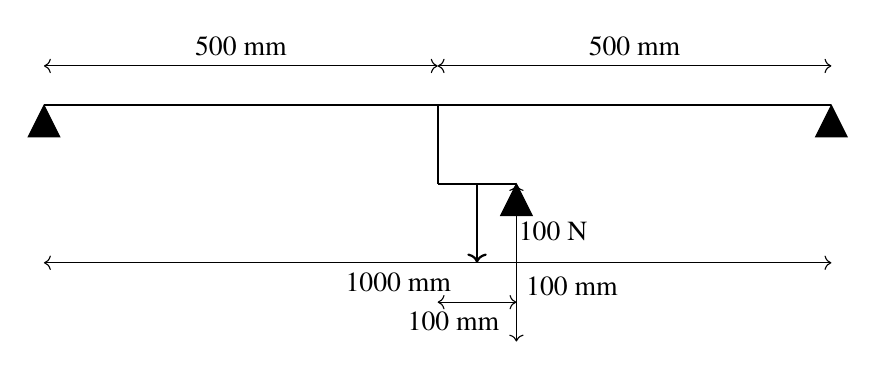
\begin{tikzpicture}
    % Beam horizontal section
    \draw[thick] (0,0) -- (10,0); % 1000 mm long beam
    
    % Beam step-down section
    \draw[thick] (5,0) -- (5,-1); % Vertical step-down 100 mm
    \draw[thick] (5,-1) -- (6,-1); % Horizontal part 100 mm
    
    % Force vector
    \draw[thick, ->] (5.5,-1) -- (5.5,-2) node[midway,right, yshift=-0.1cm, xshift= 0.4cm] {100 N}; % Downward force arrow
    
    % Supports
    \filldraw (0,0) -- (-0.2,-0.4) -- (0.2,-0.4) -- cycle; % Left triangle support
    \filldraw (10,0) -- (9.8,-0.4) -- (10.2,-0.4) -- cycle; % Right triangle support
    \filldraw (6,-1) -- (5.8,-1.4) -- (6.2,-1.4) -- cycle; % Middle triangle support at step
    
    % Dimension lines
    % Full length
    \draw[<->] (0,-2) -- (10,-2) node[midway, below, xshift=-0.5cm] {1000 mm}; 
    
    % Left section length
    \draw[<->] (0,0.5) -- (5,0.5) node[midway, above] {500 mm}; 
    
    % Right section length
    \draw[<->] (5,0.5) -- (10,0.5) node[midway, above] {500 mm}; 
    
    % Step-down horizontal length
    \draw[<->] (5,-2.5) -- (6,-2.5) node[midway, below, xshift=-0.3cm] {100 mm};
    
    % Vertical drop
    \draw[<->] (6,-1) -- (6,-3) node[midway, right, yshift=-0.3cm] {100 mm};
\end{tikzpicture}
\end{center}




\begin{multicols}{4}
\begin{enumerate}
    \item $25$
    \item $30$
    \item $35$
    \item $60$
\end{enumerate}
\end{multicols}

\item A ball bearing operating at a load $F$ has 8000 hours of life. The life of the bearing, in hours, when the load is doubled to $2F$ is

	\hfill{(GATE-ME:2007)}
\begin{multicols}{2}
\begin{enumerate}
    \item $8000$
    \item $6000$
    \item $4000$
    \item $1000$
\end{enumerate}
\end{multicols}

\item During inelastic collision of two particles, which one of the following is conserved? 

	\hfill{(GATE-ME:2007)}
\begin{multicols}{1}
\begin{enumerate}
    \item total linear momentum only
    \item total kinetic energy only
    \item both linear momentum and kinetic energy
    \item neither linear momentum nor kinetic energy
\end{enumerate}
\end{multicols}

\item A steel rod of length $L$ and diameter $D$, fixed at both ends, is uniformly heated to a temperature rise of $\Delta T$. The Young's modulus is $E$ and the coefficient of linear expansion is $\alpha$. The thermal stress in the rod is

	\hfill{(GATE-ME:2007)}
	\begin{multicols}{2}
\begin{enumerate}
    \item $0$
    \item $\alpha E \Delta T$
    \item $E \alpha \Delta T$
    \item $E \alpha \Delta T L$
\end{enumerate}
\end{multicols}
\item For an undamped harmonic oscillator, resonance 

	\hfill{(GATE-ME:2007)}

\begin{enumerate}
    \item occurs when excitation frequency is greater than undamped natural frequency
    \item occurs when excitation frequency is less than undamped natural frequency
    \item occurs when excitation frequency is equal to undamped natural frequency
    \item never occurs
\end{enumerate}

\item If a particular Fe-C alloy contains less than 0.83\% carbon, it is called

	\hfill{(GATE-ME:2007)}
	\begin{multicols}{2}
\begin{enumerate}
    \item high speed steel
    \item hypoeutectoid steel
    \item hypereutectoid steel
    \item cast iron
\end{enumerate}
\end{multicols}

\item Which of the following engineering materials is the most suitable candidate for hot chamber die casting? 

	\hfill{(GATE-ME:2007)}
	\begin{multicols}{2}
\begin{enumerate}
    \item low carbon steel
    \item titanium
    \item copper
    \item tin
\end{enumerate}
\end{multicols}

\item Which one of the following is a solid-state joining process?

	\hfill{(GATE-ME:2007)}
	\begin{multicols}{2}
\begin{enumerate}
    \item gas tungsten arc welding
    \item resistance spot welding
    \item friction welding
    \item submerged arc welding
\end{enumerate}
\end{multicols}

  	
\end{enumerate}

\end{document}
